\documentclass[12pt, letterpaper]{article}
\usepackage{graphicx}
\usepackage{geometry}
\geometry{
  a4paper,
  total={170mm,257mm},
  left=20mm,
  top=20mm,
}
\usepackage[round]{natbib}

\title{Report - Effectiveness of isolation and contact tracing to control Bundibugyo virus (Ebola disease) outbreak in the Democratic Republic of the Congo}
\author{Joshua W. Lambert}

\begin{document}

\maketitle

\section{Introduction}

On May 16 2026 the World Health Organisation stated there were 246 suspected cases of Ebola virus disease caused by the Bundibugyo virus, with eight laboratory-confirmed cases in the Democratic Republic of the Congo (DRC) \citep{who2026pheic}. Two cases have also been confirmed in Kampala, Uganda. Both individuals had travelled from the DRC \citep{who2026pheic}. However, there is likely an underascertainment of the total cases involved in the Bundibugyo virus outbreak, with a Imperial report estimating the outbreak size on 18 May 2026 was likely 400 - 800 cases in the DRC, with a possibility of more than 1,000 cases \citep{mccabe2026estimation}. A second analysis of the true outbreak size using a joint modelling approach finds the most likely total number of Ebola cases to be 450 (90\% CrI 282 - 1280) \citep{abbott2026bvdoutbreaksize}. On May 17 the WHO declared the Bundibugyo virus outbreak a public health emergency of international concern (PHEIC) \citep{who2026pheic}. On May 19, the Ministries of Health for the DRC and Uganda reported: 536 suspected cases, 105 probable cases, 34 confirmed cases \citep{cdc2026ebola}. There remain only two known cases in Uganda \citep{cdc2026ebola}. \\

The Bundibugyo species of Ebola lacks licensed pharmaceutical interventions such as antivirals and vaccines, unlike the Ebola Zaire species, for which a vaccine has been approved \citep{cepi2026bundibugyo}. With strong evidence of epidemic growth from increasing suspected cases \citep{cdc2026ebola} ($R_t > 1$), Public Health and Social Measures (PHSMs), a type of non-pharmaceutical intervention, are required to bring the outbreak under control. Isolation of cases that test positive for Ebola, and tracing of their contacts is a standard response strategy for Ebola outbreaks$^6$. \\

Here we test the effectiveness and feasibility of controlling the ongoing Bundibugyo virus outbreak in the DRC using a mathematical model. We condition the outbreak to have similar dynamics from the estimated outbreak start date, assuming a single spillover event into the human population, and then activate isolation and contact tracing of cases to evaluate whether such a response, activated mid-outbreak, and without other measures, can help bring an end to the outbreak and provide an estimate to the duration of the outbreak remaining.

\section{Methods}

We use a stochastic individual-level branching process model of disease spread in the population. We assume a single index case initiates the outbreak and that transmission in the community is defined by a Negative Binomial distribution with a basic reproduction number ($R_0$) of 3 (other values of $R_0$ are tested in a sensitivity analysis in the appendix). There is little evidence to inform the individual-level heterogeneity in transmission for Bundibugyo virus. A systematic review of Ebola virus disease finds that most estimates show moderate to high heterogeneity ($k < 1$) \citep{nash2024ebola}. We use the estimate of \citet{polonsky2021novel} from the 2018-2020 Ebola epidemic in the DRC ($k = 0.27$). \\

Ebola cases are isolated after a delay from symptom onset. We model this delay from onset-to-isolation as a Gamma distribution with a mean of 5 days and a standard deviation of 2 days (other parameters of the onset-to-isolation distribution are tested in a sensitivity analysis in the appendix). Cases can be isolated earlier than the delay after symptom onset if they are traced as a contact of a known case (i.e. their infector). When a contact is traced they are isolated as soon as their infector is isolated (or after their delay from symptom onset if earlier). Isolation is assumed to reduce all further transmission ($R_0^\mathrm{iso} = 0$). We assess how contact tracing ascertainments influences the probability of bringing the outbreak under control. \\

To simulate the speed of transmission we use the incubation period of the Bundibugyo virus [find incubation period] and sample the generation time between cases by sampling from a skew normal distribution parameterised using the proportion of transmission that occurs before or after symptom onset \citep{hellewell2020feasibility}. We assume that 1\% of Bundibugyo virus transmission events occur prior to symptom onset, which is consistent with previous Ebola outbreaks, although the proportion of presymptomatic transmission for Bundibugyo is uncertain. Our epidemic model assumes a symptom-based isolation and contact tracing system. Therefore, asymptomatic cases are assumed to be missed by the intervention and continue to transmit in the community with the same transmissibility as symptomatic cases. \\

To simulate scenarios that matched the ongoing Bundibugyo virus in the DRC we conditioned our simulation to have at least 300 cases and less than 1300 cases between 3 and 5 week into the outbreak. We assume that no PHSMs (i.e. isolation of cases or contact tracing) have been active from the start of the outbreak (spillover infection) to the present (20 May 2026). Then from the present into the future we assume that individuals that are symptomatic or contact traced from a symptomatic individual are isolated to prevent further infections.

\subsection{Counterfactual without NPIs}

To isolate the effect of isolation and contact tracing, we re-ran each of the 10 accepted scenarios with the same random seed but with no NPIs ever activated. All other parameters were held at their main-analysis values. Because in the main analysis NPIs only activate after day 35, each counterfactual trajectory is identical to its conditioned counterpart up to day 35 and diverges from that point onwards, providing a paired comparison of outbreak dynamics with and without intervention.

\section{Results}

For a baseline scenario where 50\% of contacts are successfully traced we show that for outbreaks similar to the current Ebola Bundibugyo virus epidemic, the number of new cases per week is below 15 (Figure \ref{fig:WeeklyCasesNPI}).

\begin{figure}
  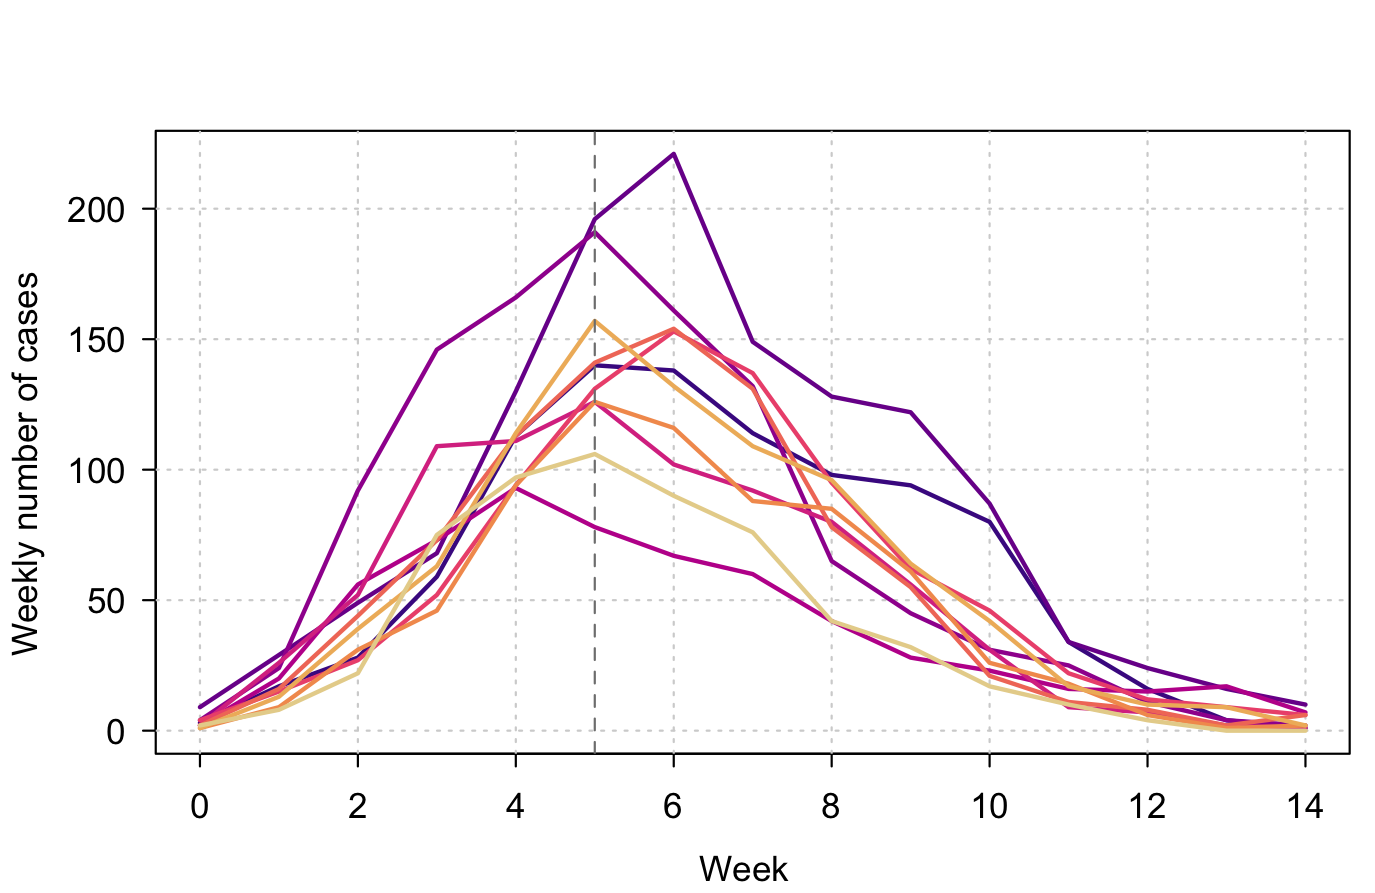
\includegraphics[width=\textwidth]{../plots/BundibugyoNPIWeeklyCases.png}
  \caption{Weekly cases of Bundibugyo virus for 10 outbreak simulations that meet the conditioning of more than 300 cases and less than 1300 cases between weeks 3-5. The dashed vertical line is the date isolation and contact tracing are activated (day 35).}
  \label{fig:WeeklyCasesNPI}
\end{figure}

However, if the highly variable (overdispersed) individual-level transmission is to be trusted then the outbreak is likely to not continue epidemic growth and instead end, without the activation of isolation and contact tracing (Figure \ref{fig:WeeklyCasesNoNPI}).

\begin{figure}
  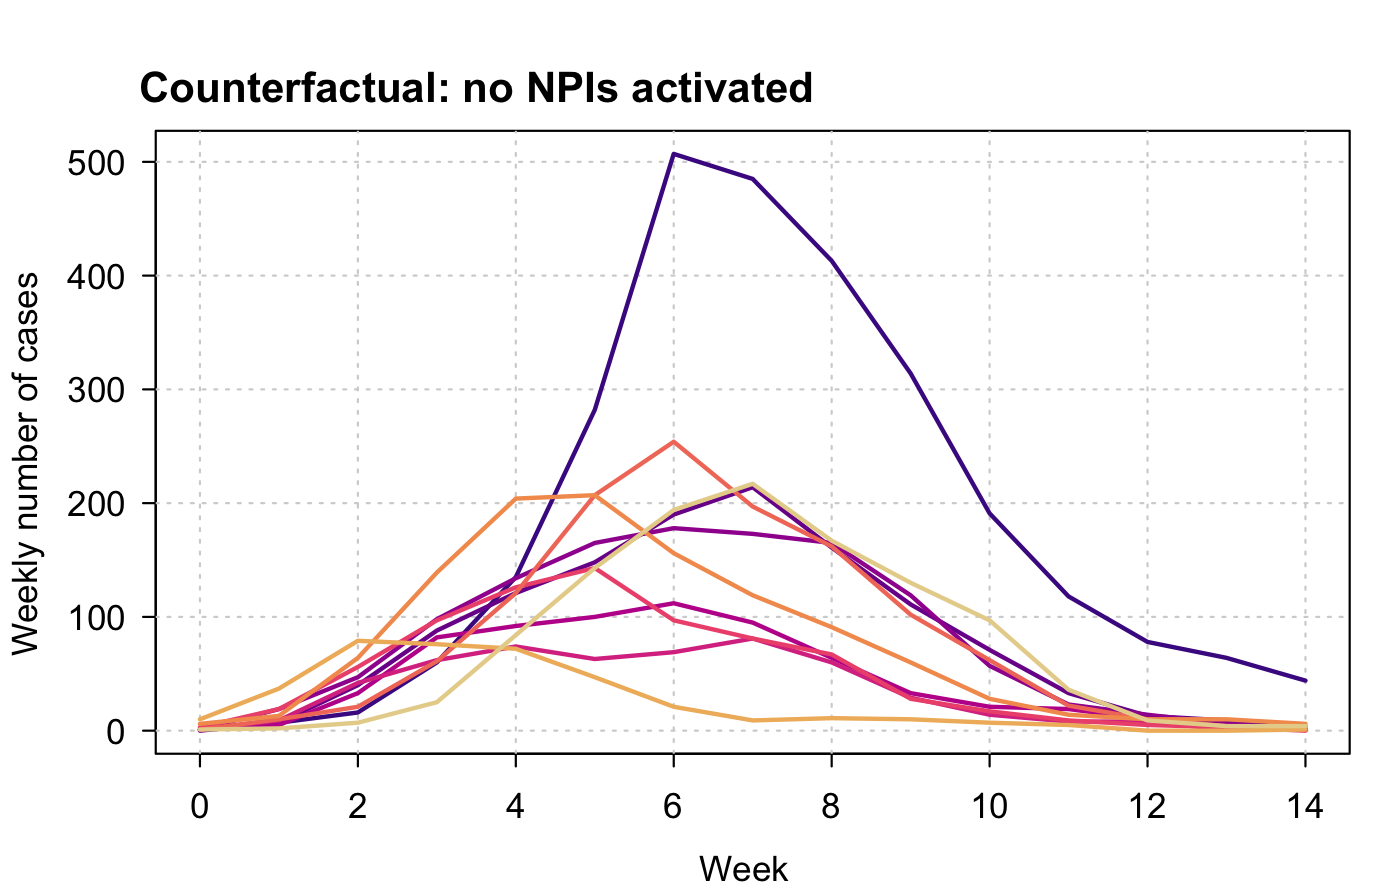
\includegraphics[width=\textwidth]{../plots/BundibugyoNoNPIWeeklyCases.png}
  \caption{Weekly cases of Bundibugyo virus for 10 outbreak simulations that meet the conditioning of more than 300 cases and less than 1300 cases between weeks 3-5. The dashed vertical line is the date isolation and contact tracing are activated (day 35).}
  \label{fig:WeeklyCasesNoNPI}
\end{figure}

\subsection{Duration of outbreak }


\section{Discussion}

\begin{itemize}
  \item Information on the transmission network would allow a better estimate of the individual-level heterogeneity in transmission, such as \cite{Althaus2015}.
\end{itemize}

\bibliographystyle{plainnat}
\bibliography{BundibugyoNPI2026.bib}

\section{Code availability}

The code to reproduce this analysis can be found at: https://github.com/joshwlambert/BundibugyoNPI2026.

The outbreak model code can be found in the R package \texttt{ringbp} at https://github.com/joshwlambert/ringbp@develop. This analysis used the \texttt{develop} branch of the ringbp package which can be installed with:

\texttt{remotes::install_github("joshwlambert/ringbp@develop")}

\section{AI Disclaimer}

This work was assisted by the use of Claude Opus 4.7.

\section{Appendix}

\subsection{Calibrating the basic reproduction number ($R_0$)}

Without a reliable estimate of the basic reproduction number ($R_0$) for Bundibugyo virus, either from the current outbreak (as of 20/05/2026) or from past outbreaks \citep{nash2024ebola}, we calibrated the community $R_0$ by sweeping it across a grid of plausible values and identifying the value most consistent with the observed early outbreak size. \\

For each value of $R_0 \in \{1.0, 1.5, 2.0, 2.5, 3.0, 3.5, 4.0\}$ we ran 10{,}000 independent branching-process simulations. All non-$R_0$ parameters were fixed to the values used in the main analysis: a Negative Binomial community offspring distribution with dispersion parameter $k = 0.27$ \citep{polonsky2021novel}, a Gamma onset-to-isolation distribution with mean 5 days and standard deviation 2 days, an asymptomatic proportion of 25\%, 1\% presymptomatic transmission, and a single index case initiating the outbreak. Isolation and contact tracing were inactive throughout the calibration window (test capacity set to zero for $t \leq 35$ days) so that the simulated trajectories reflect unmitigated transmission, mirroring the assumption in the main analysis that no PHSMs were active prior to 20 May 2026. Each simulation used an independent random seed, and seeds were reset at the start of each $R_0$ sweep, so the runs are reproducible and the sweeps for different $R_0$ values are statistically independent. \\

For each $R_0$ we recorded the proportion of simulations whose cumulative case count entered $[300, 1300]$ in any week overlapping days 21--35 of the outbreak, i.e. the same conditioning criterion as in the main analysis. The $R_0$ value yielding the highest acceptance proportion is taken as the best-supported value and is used in the main analysis; values yielding zero or near-zero acceptance over 10{,}000 runs are considered inconsistent with the observed early outbreak size. \\

The proportion of simulation iterations that met the conditioning criteria for total outbreak size during weeks 3--5 increased with increasing $R_0$.

\begin{figure}
  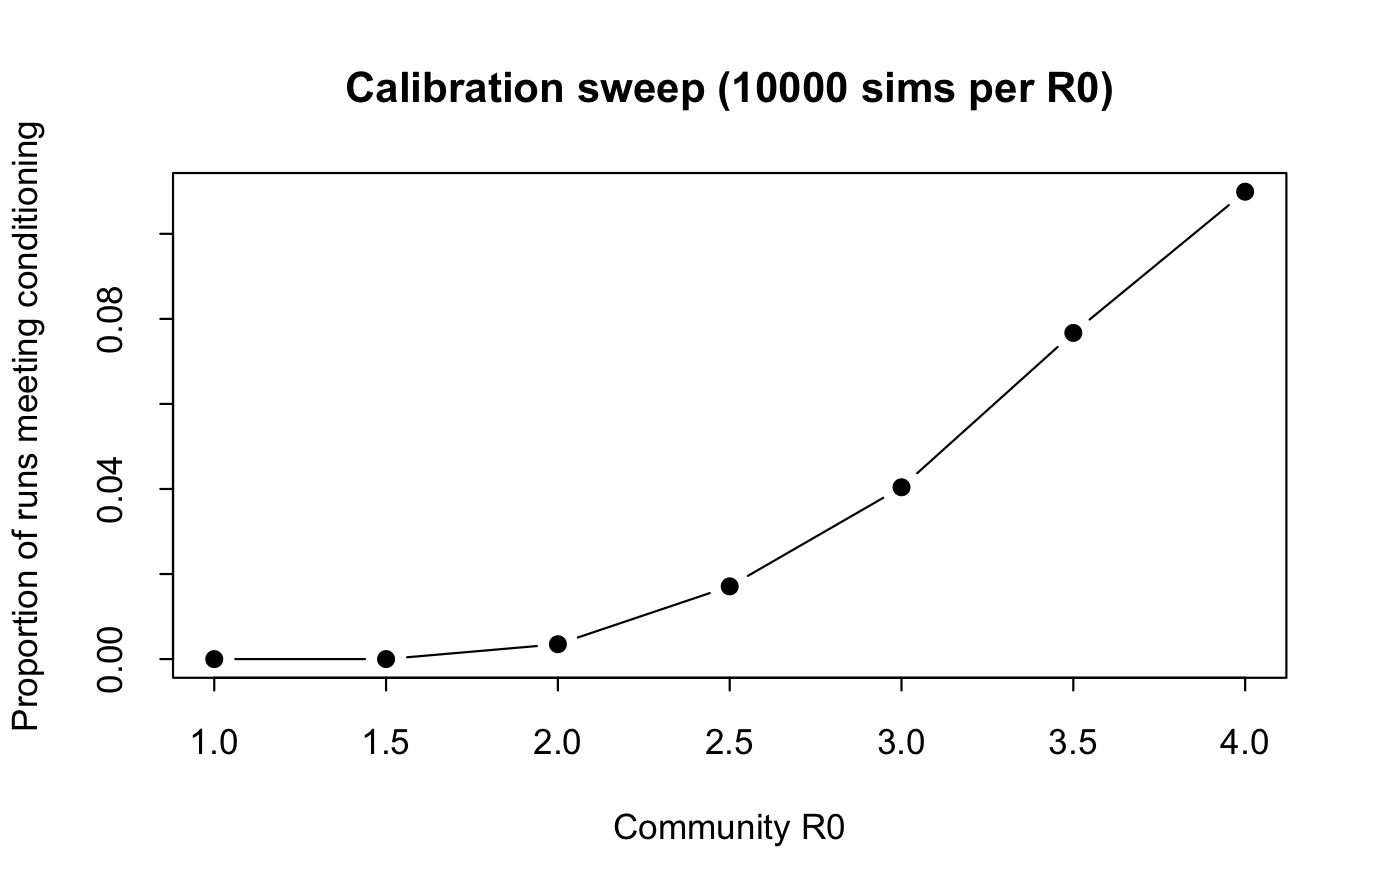
\includegraphics[width=\textwidth]{../plots/BundibugyoR0Calibration.png}
  \caption{Calibration of the community basic reproduction number ($R_0$) for Bundibugyo virus. Each point shows the proportion of 10{,}000 independent branching-process simulations whose cumulative case count entered the conditioning interval $[300, 1300]$ in at least one week overlapping days 21--35 of the outbreak, the same criterion used in the main analysis. All other parameters (offspring dispersion $k = 0.27$, onset-to-isolation distribution, asymptomatic and presymptomatic proportions, single index case, no active PHSMs) are held fixed at their main-analysis values; only the community $R_0$ varies between points. Runs are independent across $R_0$ values, with seeds reset at the start of each sweep.}
  \label{fig:R0Calibration}
\end{figure}


\end{document}
